% !TEX root = ../../report.tex

\clearpage

\section{PCB}\label{section:pcb}

While the main objective of the project is to create a MIMD system, which
essentially can be completed by FPGA design alone, everything depends on the PCB
to complete the system. This section describes everything involved with the PCB
design, and every subsection has been placed according to which stage in the
process it occurred.

\begin{figure}[H]
    \centering
    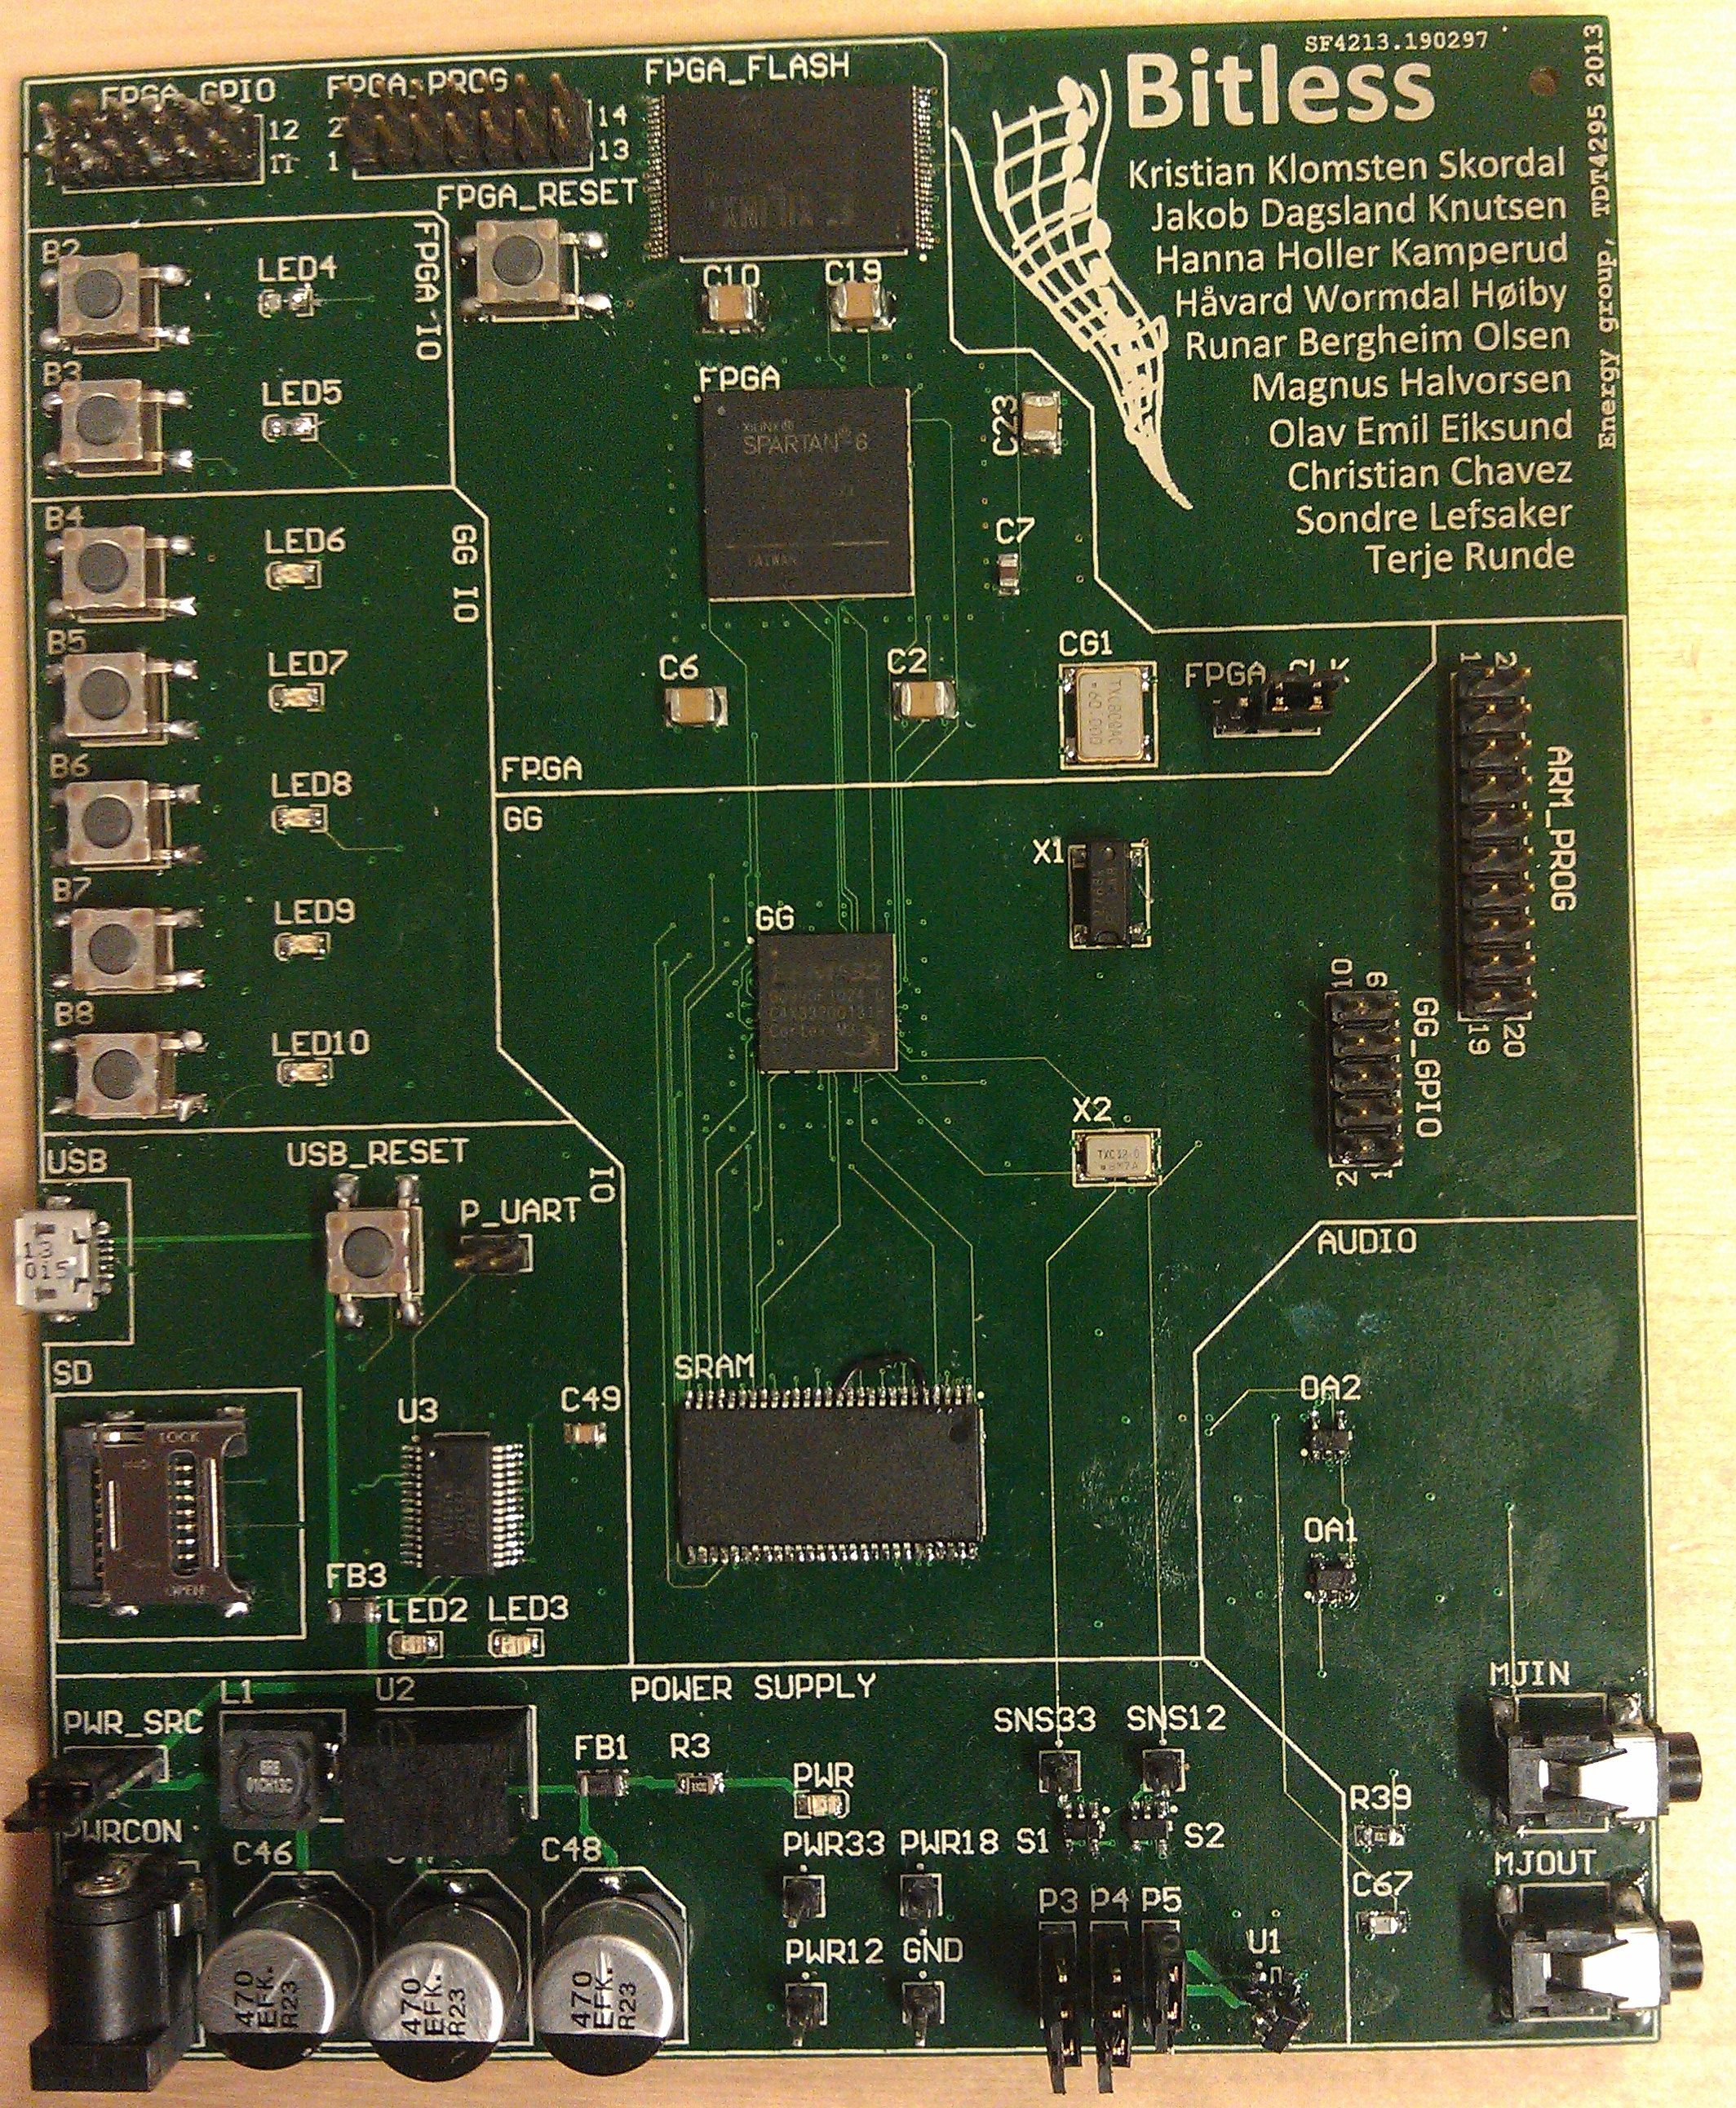
\includegraphics[scale=0.15]{figures/intro/pcb/bitless_overview}
    \caption{The Bitless computer}
    \label{fig:bitless_overview}
\end{figure}


% !TEX root = ../../report.tex

\chapter{Schematics}\label{apx:schematics}

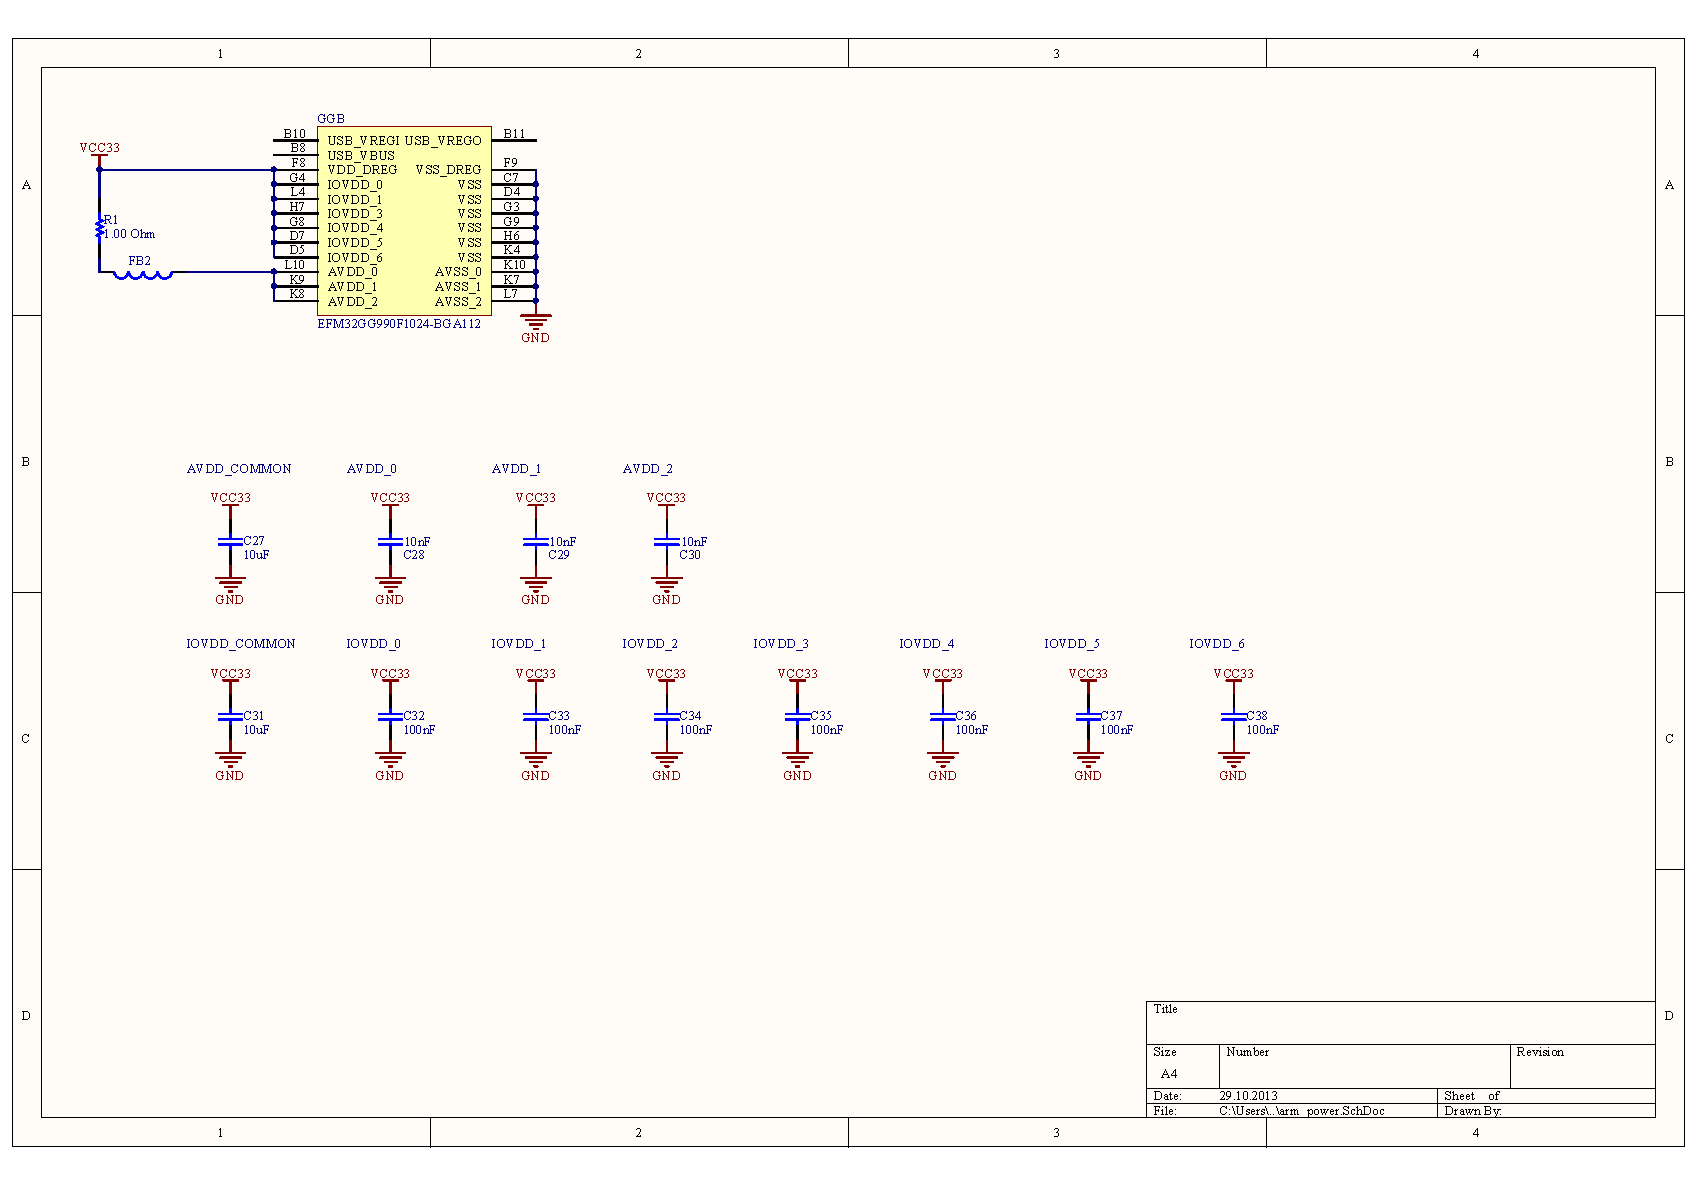
\includepdf[pages=-]{../pcb/take1/take1.pdf}
% !TEX root = ../../report.tex
\section{Components}

The PCB group was eager to learn how modern PCB production is done, using the
same tools and technologies as the industry. Thus, our choice of components was
strongly driven by a smaller is better mindset. The use of BGA packages (for
the MCU and FPGA) was already given from the resources we had available and the
fact that Odd Rune Lykkebo had experience baking these.

We used 0805 surface-mount components as much as possible, because they were the
smallest packages we could comfortably solder. This not only lowered the
production cost, but also allowed us to place components on both sides of the
board, and consequently minimizing the size.

{\bf USB-UART}
\begin{itemize}
  \item FTDI FT232RL - USB-UART converter
  \item 1x 4k7 and 1x 10k
  \item 3x 100nF and 1x 4.7uF
  \item USB3140-30-0170-1-C USB Micro B connector 
\end{itemize}


  



	

\section{Layout}
% !TEX root = ../../../../report.tex

\subsubsection{Routing}

Almost everything was autorouted, with only a few exceptions. The power supply had to be done manually, as well as the fanout on the FPGA. The routes are visible in the last image of Appendix~\ref{apx:schematics}.
% !TEX root = ../../report.tex
\section{Layer Stack}

We had three primary voltage levels on the PCB -- 1.2V, 1.8V and 3.3V. To
minimize resistance in the power distribution system, we decided to dedicate a
layer on the PCB to be used as a shared power plane. Another plane was used for
common ground and covered the whole PCB (excluding non-grounded through-holes).
This is setup with a shared ground and split power plane is common practice for
modern PCB design.

As for the signal layers, the BGA packages we used had only 0.8 mm pitch between
its feets. This forced us to have more signal layers than we originally set out
for, to be able to fanout and escape the BGA packages. Using a QFP-like package
could probably have saved us some cost, but using BGA gave us a valuable
experience on modern PCB design.

We settled upon a total of 8 layers on the PCB.

% !TEX root = ../../../../report.tex
\subsubsection{Footprints}

Each component is associated with a schematic drawing and a footprint. Because certain components were not available in public libraries they had to be drawn from scratch. Below is a list of all custom drawings and footprints.

\begin{table}[h]
	\centering
	\begin{tabular}{|l l l|}
		\hline
		\textbf{Component} & \textbf{Footprint}  & \textbf{Schematic} \\
		\hline
		XP Power Switch-Mode Regulator & X & X \\
		Würth Electronics MicroSD & X & X \\
		Molex MicroUSB AB & X & X \\
		Lumberg 3.5mm audio jack & X & X \\
		Buttons & X & X \\
		DC-10B & X & X \\
		Texas Instruments Op amp & X & X \\
		Diodes INC. Linear regulator& X & X \\
		Cypress Semiconductor SRAM & X & X \\
		& X & X \\
		& X & X \\
		& X & X \\
		& X & X \\
		\hline
	\end{tabular}
	\caption{Custom footprints and schematics}
	\label{tab:footprints}
\end{table}

\todo{finish table}

% !TEX root = ../../../../report.tex

\subsubsection{Programming Interfaces}

\paragraph{FPGA Programming}
The FPGA can be programmed in numerous configurations, all of which have
distinct features and capabilities described in the \todo{insert reference?}
Spartan-6 FPGA Configuration User Guide. To avoid ruining the programmability, a
decision was made to go for the simplest and less error-prone configuration; a
JTAG interface directly to the chip.

However, JTAG programming does not provide persistence -- the FPGA would have to
be reprogrammed every time it powered up. This was not an ideal solution, so a
FPGA configuration flash memory was added, from which the FPGA could read its
initial configuration at startup. Xilinx provides schematics to daisy-chain the
regular JTAG with a JTAG interface to the FPGA flash, making it easy to
implement. Using this setup both the FPGA and the flash will be programmed
simultaneously, and unlike the FPGA the flash will retain the program when
powered down. When powered up again the FPGA will look to the flash for its
initial program.

\paragraph{MCU Programming}
Placing programming headers for the MCU on the PCB is a much simpler procedure.
The 20-pin ARM debug pinout is well documented in application notes and is
simple to set up.

In addition to programming the MCU, the debug header permits tracing of running
programs, as well as allowing the use of the energy profiler provided by Silicon Labs.
